\subsection{把规则放回真正的约束反演以后}
我还固定四个代表对象，把receiver和exchange放进相同的outer reconstruction：同一初始化、prior、LM schedule、材料可行域以及完整非线性目标上的Armijo line search，只改变切向电流策略。三个完整对照都完成18次接受更新。平滑voxel、近接触Gaussian和shell Gaussian的复材料相对误差分别从0.3027、0.6722、0.6096降到0.2699、0.6707、0.5660，约下降10.8\%、0.22\%、7.16\%。留出测量误差也均下降。

这里有一个值得正面解释的差别：近接触对象的数据拟合改善很明显，但复材料改善很小，实部还略差。这使我更明确地区分“更忠实的完整GN步”和“更好的材料估计”。第四个非对称voxel对象的exchange轨迹保留17次已完成更新。在第18次更新前，它为开始当次交换构建的receiver endpoint没有通过残差验收，因而停止；独立的receiver-only基线轨迹尚未运行。我保留这组未形成完整对照的结果，没有放宽验收条件。

每条轨迹独立计入setup、acquisition、line search和最终评价后，exchange耗时是receiver的2.68、1.74、1.46倍。它支付了额外的$Jd$作用，换取更新保真度，而不是更快的成像。我的论文因此以Maxwell机制和conditional design为主，把这三组重建作为有限的secondary consequence。

\begin{figure}[htbp]\centering
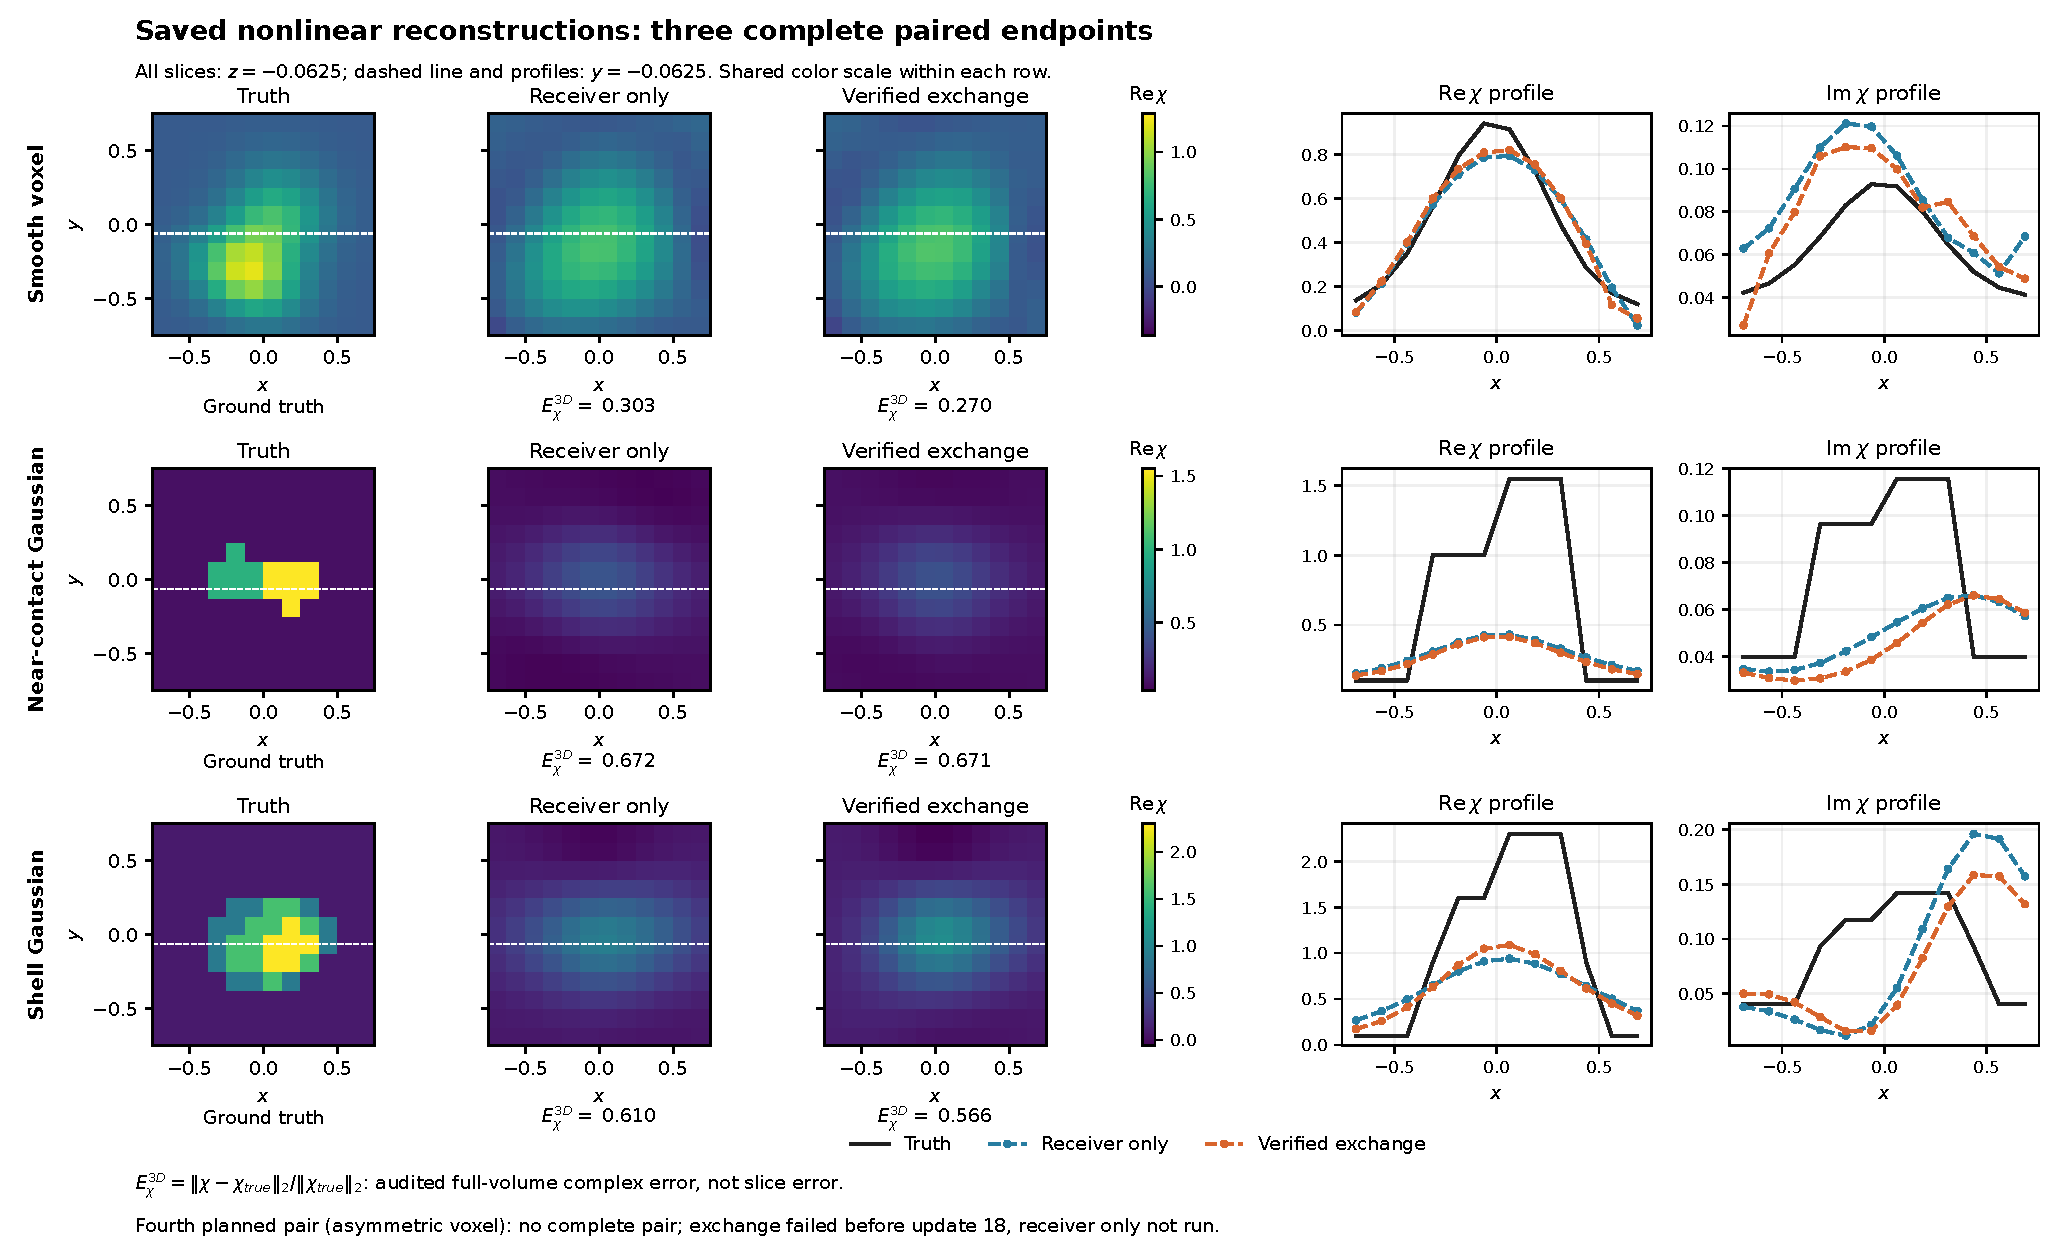
\includegraphics[width=.95\linewidth]{figures/nonlinear_closure_v1/nonlinear_reconstructions.pdf}
\caption{三组完整对照的材料切片与剖面。每行共用色标，曲线同时展示实部和虚部；完整误差用整个三维材料计算。近接触及shell结构的峰值和界面仍不清晰，数据拟合改善没有自动解决材料辨识。}
\end{figure}
